\documentclass[9pt]{extarticle}
\usepackage[twocolumn,letterpaper,margin=0.68in,columnsep=0.28in]{geometry}
\usepackage{mathptmx}
\usepackage[T1]{fontenc}
\usepackage{amsmath,amssymb}
\usepackage{booktabs}
\usepackage{array}
\usepackage{graphicx}
\usepackage{xcolor}
\usepackage{caption}
\usepackage[hidelinks,colorlinks=false]{hyperref}
\usepackage{titlesec}
\usepackage{enumitem}
\setlist{nosep,leftmargin=1.1em}

\captionsetup{font=small,labelfont=bf,skip=3pt}
\titlespacing*{\section}{0pt}{6pt}{3pt}
\titlespacing*{\subsection}{0pt}{5pt}{2pt}
\renewcommand{\arraystretch}{1.0}
\setlength{\textfloatsep}{6pt plus 1pt minus 2pt}
\setlength{\intextsep}{5pt plus 1pt minus 2pt}
\setlength{\floatsep}{5pt plus 1pt minus 2pt}
\setlength{\abovecaptionskip}{3pt}
\setlength{\belowcaptionskip}{0pt}

\titleformat{\section}{\normalfont\fontsize{10.5}{12}\bfseries}{\thesection}{0.6em}{}
\titleformat{\subsection}{\normalfont\fontsize{9.5}{11}\bfseries\itshape}{\thesubsection}{0.6em}{}

\newcommand{\pval}[1]{\ensuremath{p = #1}}

\begin{document}

\twocolumn[
\begin{center}
{\Large\bfseries Where Mixing Activations Helps: A Hidden-Width Sweep of
Tanh+ReLU Hybrid Hidden Layers on MNIST}\par\vspace{7pt}
{\normalsize Barkev}\par\vspace{2pt}
{\small\itshape Independent study}\par\vspace{10pt}
\end{center}
\begin{quote}\small
\textbf{Abstract.} We revisit the claim that mixing activation functions
\emph{within} a hidden layer -- assigning some neurons \texttt{tanh} and the
rest \texttt{ReLU} -- improves classification accuracy. An earlier,
uncontrolled version of this experiment reported a 6.5-point advantage for
the hybrid, which we show was an artefact of an unstable homogeneous-ReLU
baseline. Under a corrected protocol (uniform output layer, per-configuration
learning-rate calibration, a fixed data split, and paired evaluation across
shared seeds) on a \(784\text{-}H\text{-}H\text{-}10\) MLP trained with
batch-size-1 SGD, we sweep the hidden width \(H \in \{12,32,64,128,256,512\}\)
with 5--30 seeds per configuration and compare \texttt{relu}, \texttt{tanh},
and the interleaved \texttt{tanh+relu} hybrid. The hybrid's advantage over
\texttt{relu} is not constant: it is significantly \emph{negative} at
\(H{=}12\) (\(-0.57\) points, \pval{5.5\mathrm{e}{-6}}) and \(H{=}32\)
(\(-0.18\), \pval{5.6\mathrm{e}{-4}}), crosses zero between \(H{=}32\) and
\(H{=}64\), and is the best-performing configuration at \(H \geq 64\), reaching
\(+0.23\) points at \(H{=}256\) (\pval{0.071}). A second, statistically
sharper effect is that the hybrid is far more tolerant of an aggressive
learning rate: at \(H{=}12\), \texttt{relu} collapses to chance accuracy at
\(\mathrm{lr}=0.1\) while \texttt{tanh+relu} keeps training normally. We
report the crossover, the robustness effect, a negative result on activation
layout and mixing ratio, and the sample-size and split-portability
limitations that qualify all of the above.
\end{quote}
\vspace{4pt}
]

\section{Introduction}
Networks that mix more than one activation function inside a single hidden
layer -- rather than using one function uniformly -- have been proposed
informally as a way to get some of the sparsity benefits of ReLU-family
units together with the bounded, always-differentiable gradient of
\texttt{tanh} or \texttt{sigmoid}. An earlier version of this codebase tested
exactly this idea with an even/odd neuron split and reported a large win for
\texttt{tanh+relu} over homogeneous \texttt{relu} (86.3\% vs.\ 92.9\% mean
test accuracy across 232 seeds). That comparison, however, also hybridised
the \emph{output} layer, used mean-squared error with a single, untuned
learning rate, and had no \texttt{tanh}-only baseline -- so it could not
separate ``hybridisation helps'' from ``the ReLU baseline was badly tuned.''

This paper re-runs the comparison with those confounds removed and asks a
narrower, better-posed question: \emph{as a function of hidden width, does an
interleaved tanh+relu hidden layer beat its homogeneous parents on a held-out
test set, and if the answer changes sign, where and why?} We find that it
does change sign, we locate the crossover between widths 32 and 64, and we
show that the width trend in raw accuracy is accompanied by a separate and
more robust effect on learning-rate tolerance that plausibly explains why a
badly-tuned baseline can make hybrids look better than they are.

\section{Method}

\subsection{Architecture and activation masks}
All experiments use a fully connected \(784 \rightarrow H \rightarrow H
\rightarrow 10\) network (MNIST, \(28\times28\) grayscale digits) trained
with plain batch-size-1 SGD (no momentum, no batch normalization), Kaiming-uniform
weight initialization (bound \(\sqrt{1/\mathrm{fan\_in}}\), matching the
default used by PyTorch's \texttt{nn.Linear}), and a gradient clip of
\(\pm 10\) on the pre-activation error signal. Both hidden layers are given a
per-neuron activation mask: for a homogeneous configuration every neuron uses
the same function; for a hybrid, neurons alternate between \texttt{act1} and
\texttt{act2} as evenly as possible (\emph{interleave} layout, mix ratio
0.5), which reproduces the even/odd split used by the original, uncontrolled
experiment. The output layer is always homogeneous -- linear units with a
softmax and cross-entropy loss for all main results, so that hybridisation is
isolated to the hidden layers and cannot be confounded with output-layer
effects as it was previously.

\subsection{Data and evaluation}
All experiments train on the standard 60,000-image MNIST training file, split
once into 45,000 training / 5,000 validation / 10,000 test examples with a
fixed permutation (seeded, independent of the per-run seed) that is identical
for every configuration and width. Ten epochs of training are used
throughout. We report test-set accuracy and macro-averaged F1 (over the
10-class confusion matrix) at the end of training; validation accuracy is
also tracked every epoch and used only for learning-rate selection, never for
model selection among seeds.

\subsection{Learning-rate calibration}
Because a fixed learning rate systematically favors whichever activation
tolerates it best, we select a learning rate per (configuration, width) pair
from the grid \(\{0.001, 0.003, 0.01, 0.03\}\) by mean validation accuracy
over three held-out calibration seeds (101--103) that are never reused for
evaluation. Calibrated rates rise with width for the hybrid and for
\texttt{tanh} (0.003 at \(H{\le}32\), 0.01 from \(H{=}64\) up) while staying
at 0.003 for \texttt{relu} at every width except 512; this is a real part of
the comparison; it is not a source of unfairness we removed, and we flag
below where it matters for interpretation.

\subsection{Seeds and statistics}
Every configuration at a given width is evaluated on the same set of seeds
(1--30 at \(H{=}12,32\); 1--20 at \(H{=}64,128\); 1--10 at \(H{=}256\); 1--5
at \(H{=}512\), reflecting compute available for the sweep), so seed \(i\)'s
train/val/test split, per-epoch shuffling, and weight initialization line up
across configurations and all comparisons are paired. For each comparison we
report the mean paired difference, a 95\% bootstrap confidence interval
(10,000 resamples), a paired \(t\)-test \(p\)-value, and a Wilcoxon
signed-rank \(p\)-value as a distribution-free check; we do not apply a
multiple-comparisons correction, and say explicitly, in \S\ref{sec:limits},
which individual \(p\)-values would and would not survive one.

\section{Results}

\subsection{Accuracy against width}
Table~\ref{tab:main} and Figure~\ref{fig:width} give test accuracy for
\texttt{relu}, \texttt{tanh}, and \texttt{tanh+relu} at each width. All three
configurations improve steeply from \(H{=}12\) to \(H{=}64\) and then
flatten: the width-to-width gain for \texttt{relu} shrinks monotonically from
\(+2.73\) points (12\(\to\)32) to \(+0.10\) points (256\(\to\)512), consistent
with MNIST's accuracy ceiling rather than with any activation-specific
effect. \texttt{tanh} is the weakest of the three at every width tested.
\texttt{relu} leads at \(H{=}12\) and \(32\); \texttt{tanh+relu} leads at
every width from 64 upward, and is the best single configuration overall at
\(H{=}256\) (98.14 $\pm$ 0.16) and ties its own \(H{=}512\) result (98.14 $\pm$
0.14).

\begin{table}[t]
\centering\small
\caption{Test accuracy (mean $\pm$ sd, \%) by hidden width $H$ and number of
seeds $n$ per configuration.}
\label{tab:main}
\begin{tabular}{@{}lrrrr@{}}
\toprule
$H$ & $n$ & relu & tanh & tanh+relu \\
\midrule
12  & 30 & \textbf{93.72 $\pm$ 0.49} & 93.32 $\pm$ 0.27 & 93.15 $\pm$ 0.47 \\
32  & 30 & \textbf{96.45 $\pm$ 0.26} & 96.19 $\pm$ 0.25 & 96.27 $\pm$ 0.20 \\
64  & 20 & 97.19 $\pm$ 0.20 & 97.11 $\pm$ 0.12 & \textbf{97.22 $\pm$ 0.23} \\
128 & 20 & 97.75 $\pm$ 0.14 & 97.70 $\pm$ 0.15 & \textbf{97.83 $\pm$ 0.18} \\
256 & 10 & 97.92 $\pm$ 0.31 & 97.84 $\pm$ 0.14 & \textbf{98.14 $\pm$ 0.16} \\
512 & 5  & 98.02 $\pm$ 0.21 & 97.74 $\pm$ 0.11 & \textbf{98.14 $\pm$ 0.14} \\
\bottomrule
\end{tabular}
\end{table}

\begin{figure}[t]
\centering
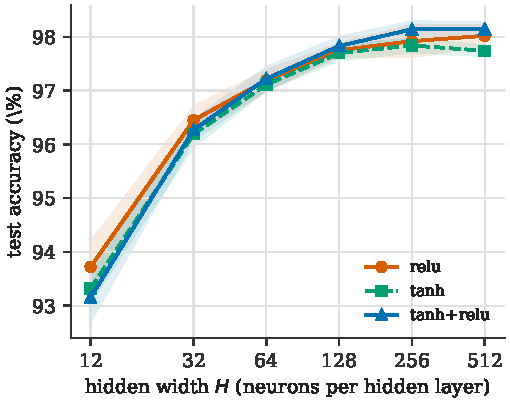
\includegraphics[width=\linewidth]{figs/fig1_accuracy_vs_width.pdf}
\caption{Test accuracy against hidden width for the three configurations.
Shaded bands are $\pm1$ sd over seeds. Gains shrink at every width
doubling, consistent with approaching MNIST's accuracy ceiling.}
\label{fig:width}
\end{figure}

\subsection{The crossover}
Table~\ref{tab:crossover} and Figure~\ref{fig:crossover} report the paired
difference \texttt{tanh+relu} $-$ parent directly, which is the quantity that
actually matters: raw accuracy differences are small everywhere, but the
paired design turns them into narrow, mostly non-overlapping confidence
intervals. Against \texttt{relu}, the hybrid is significantly \emph{worse} at
\(H{=}12\) and \(32\) (both intervals exclude zero and survive a Bonferroni
correction across the twelve tests in this table, threshold
\(0.05/12 \approx 0.0042\)), statistically indistinguishable from \texttt{relu}
at \(H{=}64\) and \(128\), and nominally ahead at \(H{=}256\) and \(512\), though
neither of those two intervals excludes zero and neither $p$-value survives
correction. Against \texttt{tanh}, the hybrid's advantage is more consistent
in sign (positive from \(H{=}32\) up) and grows with width, reaching
significance uncorrected at \(H{=}64\), \(128\), \(256\), and \(512\) (the
last of these is a within-subjects sweep at 5/5 seeds), but again none of the
\(H\geq 64\) comparisons survives the Bonferroni threshold. We treat the
\(H{=}12\) and \(32\) losses against \texttt{relu} as the one part of this
result that is not in doubt, and the \(H\geq 64\) hybrid advantage as a
consistent trend worth confirming with more seeds rather than a settled
finding.

\begin{table}[t]
\centering\small
\caption{Paired \texttt{tanh+relu} $-$ parent, test accuracy (points). CI is
the 95\% bootstrap interval of the mean difference; wins counts seeds where
the hybrid scored higher.}
\label{tab:crossover}
\begin{tabular}{@{}lrrrl@{}}
\toprule
$H$ & $\Delta$ vs relu & 95\% CI & wins & $p$ (paired $t$) \\
\midrule
12  & $-$0.57 & [$-$0.77,$-$0.38] & 4/30 & 5.5e-06 \\
32  & $-$0.18 & [$-$0.27,$-$0.09] & 7/30 & 5.6e-04 \\
64  & +0.03 & [$-$0.07,+0.13] & 11/20 & 0.640 \\
128 & +0.08 & [$-$0.02,+0.18] & 14/20 & 0.159 \\
256 & +0.23 & [+0.03,+0.43] & 8/10 & 0.071 \\
512 & +0.12 & [$-$0.14,+0.38] & 3/5 & 0.476 \\
\midrule
$H$ & $\Delta$ vs tanh & 95\% CI & wins & $p$ (paired $t$) \\
\midrule
12  & $-$0.17 & [$-$0.35,+0.01] & 10/30 & 0.084 \\
32  & +0.08 & [$-$0.01,+0.16] & 18/30 & 0.084 \\
64  & +0.11 & [+0.01,+0.22] & 13/20 & 0.057 \\
128 & +0.13 & [+0.03,+0.22] & 16/20 & 0.020 \\
256 & +0.30 & [+0.15,+0.45] & 8/10 & 0.004 \\
512 & +0.40 & [+0.32,+0.53] & 5/5 & 0.003 \\
\bottomrule
\end{tabular}
\end{table}

\begin{figure}[t]
\centering
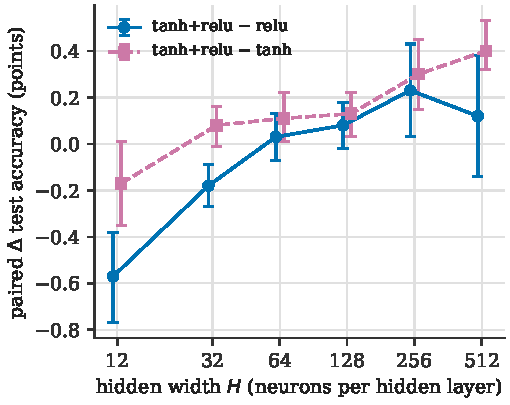
\includegraphics[width=\linewidth]{figs/fig2_crossover.pdf}
\caption{Paired difference (hybrid $-$ parent) against width, with 95\%
bootstrap CIs. The hybrid loses to \texttt{relu} at low width, crosses zero
between $H{=}32$ and $H{=}64$, and leads from $H{=}64$ up; the advantage over
\texttt{tanh} is positive and widening from $H{=}32$ on.}
\label{fig:crossover}
\end{figure}

\subsection{Why does the width-512 effect look weaker than width-256?}
\label{sec:hantallasma}
One natural reading of Table~\ref{tab:crossover} is that the hybrid's
advantage peaks at \(H{=}256\) (+0.23, \pval{0.071}) and then shrinks at
\(H{=}512\) (+0.12, \pval{0.476}), and one might attribute this to the larger
network becoming harder to optimize -- more parameters, a longer, noisier
path to a good minimum. Two observations argue against that reading. First,
the train/test accuracy gap, which is where an optimization or capacity
problem would show up, does not widen from \(H{=}256\) to \(H{=}512\): it is
1.66 points for \texttt{relu} and 1.54 for \texttt{tanh+relu} at \(H{=}256\),
versus 1.58 and 1.50, respectively, at \(H{=}512\) -- if anything slightly
tighter. Training accuracy itself is flat at 99.5--99.7\% from \(H{=}128\)
onward for all three configurations, so the network is not struggling to fit
the training set at the larger width. Second, the standard error of the
paired difference is consistent with a pure sample-size effect: it is
\(\approx\)0.10 points at \(H{=}256\) (\(n{=}10\)) and \(\approx\)0.13 at
\(H{=}512\) (\(n{=}5\)), and \(0.10\times\sqrt{10/5}\approx0.14\) is close to
the observed value. In other words, halving the seed count is sufficient by
itself to explain most of the loss of significance, without needing to posit
that the underlying effect became smaller or that the larger network is
harder to train. What is real and uncontroversial is that both accuracy
\emph{and} the size of further accuracy gains are running into a ceiling as
\(H\) grows on a dataset as easy as MNIST; what is not established by this
data is that \(H{=}512\) is a qualitatively different, harder-to-optimize
regime for these networks specifically. Table~\ref{tab:main} is consistent
with a saturating task, not with a sluggish network.

\subsection{Learning-rate robustness}
The most statistically unambiguous effect in this study is not about
accuracy at the tuned learning rate at all: it is about what happens away
from it. At \(H{=}12\), raising the learning rate from the calibrated 0.003
to 0.1 collapses \texttt{relu} to 11.3\% mean validation accuracy (10/10
seeds below the 50\% collapse threshold, chance being 10\%), while
\texttt{tanh+relu} is still at 76.3\% (0/10 seeds collapsed) and
\texttt{tanh} at 78.7\% (Figure~\ref{fig:lr}). This reproduces, with a
mechanism, the original uncontrolled result: a homogeneous ReLU network run
at too high a learning rate looks catastrophically worse than a hybrid, and
if the comparison never calibrates the learning rate per configuration, that
gap is mistaken for an accuracy effect rather than a stability effect. The
effect is width-dependent in a way that also constrains how far the claim
generalizes: at \(H{=}128\) the same 0.1 learning rate collapses
\texttt{tanh+relu} on 8/10 seeds (mean 30.2\%) and \texttt{relu} on 8/10
(mean 11.8\%) -- the hybrid is less dead than \texttt{relu} but is not
robust in the way it is at \(H{=}12\). \texttt{leaky\_relu}, which we ran as
an additional homogeneous baseline, does not collapse at either width at any
tested learning rate up to 0.3, indicating that a non-zero negative branch is
what confers robustness in general, and mixing in \texttt{tanh} only
partially substitutes for it, and only in the narrower network.

\begin{figure}[t]
\centering
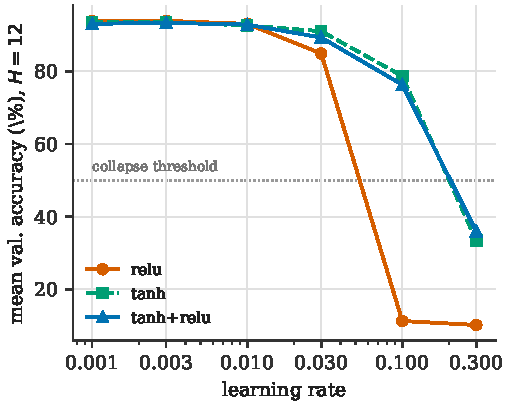
\includegraphics[width=\linewidth]{figs/fig3_lr_robustness.pdf}
\caption{Mean validation accuracy against learning rate at $H{=}12$ (10
seeds per point). \texttt{relu} collapses to chance beyond
$\mathrm{lr}=0.03$; the hybrid tracks \texttt{tanh}'s tolerance.}
\label{fig:lr}
\end{figure}

\subsection{Where the tanh neurons sit does not matter}
At \(H{=}12\) and \(H{=}128\) we compared the default interleaved, ratio-0.5
mask against a block layout (all \texttt{tanh} neurons first), a random
shuffle of the block mask, and interleaved masks at ratios 0.25 and 0.75.
Every variant at \(H{=}128\) lands within 0.15 points of interleave/0.5 with
signs that do not reproduce across width (the ratio-0.75 variant is the
weakest layout at \(H{=}128\) but the strongest at \(H{=}256\)), which is the
signature of noise rather than a real placement effect. We take this as a
negative result: at the widths tested, \emph{how many} of a layer's units are
\texttt{tanh} and \emph{which} units they are do not measurably change test
accuracy once the better parent's learning rate is (re-)used; layout is not
where the crossover in \S3.2 lives.

\section{Discussion}
The overall picture is two effects that point in different directions and
should not be collapsed into one number. First, a small but real
\emph{crossover}: mixing \texttt{tanh} into a \texttt{relu} hidden layer
costs accuracy in narrow networks and gains a little in wider ones, most
plausibly because in a 12- or 32-unit layer every unit's representational
contribution matters and a \texttt{tanh} unit is, on this task, simply a
slightly worse feature detector than a \texttt{relu} unit, while a wider
layer has enough redundant capacity that a fraction of bounded,
always-differentiable units becomes a net positive rather than a tax. Second,
a \emph{robustness} effect that is much larger in relative terms and far more
statistically secure at \(H{=}12\): whatever headroom the hybrid gives up in
its best case at low learning rate, it more than gets back the moment the
learning rate is even mildly mistuned. This second effect is, in our view,
the actual explanation for the original 6.5-point result that motivated this
study -- not because hybridisation is a better function approximator, but
because an untuned, homogeneous ReLU network is a fragile baseline to compare
against.

\section{Limitations}
\label{sec:limits}
Several limitations qualify every number above. \textbf{(i) Sample size at
the extremes.} The \(H{=}512\) condition has 5 seeds per configuration, and
its confidence intervals are correspondingly wide; \S\ref{sec:hantallasma}
argues this, not a genuine optimization difficulty, is why its effect looks
weaker than \(H{=}256\)'s. \textbf{(ii) Multiple comparisons.} Table~2
reports twelve paired tests without correction; only the \(H{=}12\) and
\(H{=}32\) losses to \texttt{relu} survive a Bonferroni threshold of
\(0.05/12\), and the \(H\geq64\) wins over \texttt{relu} and \texttt{tanh}
should be read as suggestive, not confirmatory. \textbf{(iii) Split
portability.} The fixed 45k/5k/10k split is generated by
\texttt{std::shuffle} from a fixed seed, but the C++ standard does not
guarantee that \texttt{std::shuffle} produces the same permutation across
standard-library implementations; we verified directly that data produced on
a different machine/toolchain used a demonstrably different split (different
per-class test-set counts from the same seed) and is therefore not
row-comparable with the results reported here. All results in this paper
come from a single machine and a single compiled binary, so this does not
affect internal validity, but it means the exact accuracy numbers are not
expected to reproduce bit-for-bit elsewhere even with the same source code
and seeds. \textbf{(iv) Single dataset, single architecture family.} All
results are on MNIST with a 2-hidden-layer MLP trained by plain SGD; we make
no claim about convolutional architectures, other datasets, or optimizers
with momentum or adaptive learning rates. \textbf{(v) One hybrid pairing as
the main subject.} We also collected data for \texttt{tanh+leaky\_relu},
\texttt{sigmoid}, and \texttt{sigmoid+relu} homogeneous and hybrid baselines;
the width effect reported here is specific to \texttt{tanh+relu} and does not
replicate for \texttt{tanh+leaky\_relu}, whose hybrid-parent difference is
not monotonic in width and is negative at \(H{=}512\) ($-0.21$, 0/5 seeds).

\section{Conclusion}
Under a controlled protocol, mixing \texttt{tanh} and \texttt{relu} within a
hidden layer is not a uniform accuracy improvement: it costs 0.2--0.6 points
in narrow (12--32 unit) hidden layers and gains a similar amount, though less
certainly, in wider (64--512 unit) ones, crossing zero between \(H{=}32\) and
\(H{=}64\) on MNIST. The more reliable effect is that the hybrid tolerates a
poorly chosen learning rate far better than homogeneous \texttt{relu} does at
small width, which is almost certainly the real mechanism behind the
uncontrolled result that motivated this study. Future work that would
directly extend this analysis: more seeds at \(H{=}512\) to determine whether
the hybrid's lead over \texttt{relu} there is genuine; a finer width grid
between 32 and 64 to localize the crossover; a principled, dead-unit-aware
rule for which neurons should be \texttt{tanh} rather than an index-based
mask, since \S3.5 shows the current placement rule does not matter; and
replication on a second dataset such as Fashion-MNIST or CIFAR-10, for which
a data loader already exists in this codebase.

\vspace{2pt}
{\small\noindent\textbf{Reproducibility.} All training code, sweep scripts,
raw per-seed CSVs (22 fields including the full test confusion matrix), and
the analysis script that generates every table and figure in this paper are
in the \texttt{version5/} directory of the project repository. Seeds 1--30
are shared across every configuration at a given width, so every comparison
in this paper can be recomputed from the raw CSVs without retraining.}

\begin{thebibliography}{9}\small
\setlength{\itemsep}{0pt}

\bibitem{lecun1998} Y.\ LeCun, L.\ Bottou, Y.\ Bengio, and P.\ Haffner.
``Gradient-based learning applied to document recognition.''
\emph{Proceedings of the IEEE}, 86(11):2278--2324, 1998.

\bibitem{nair2010} V.\ Nair and G.\ E.\ Hinton. ``Rectified linear units
improve restricted Boltzmann machines.'' In \emph{Proc.\ ICML}, 2010.

\bibitem{glorot2010} X.\ Glorot and Y.\ Bengio. ``Understanding the
difficulty of training deep feedforward neural networks.'' In \emph{Proc.\
AISTATS}, 2010.

\bibitem{maas2013} A.\ L.\ Maas, A.\ Y.\ Hannun, and A.\ Y.\ Ng. ``Rectifier
nonlinearities improve neural network acoustic models.'' In \emph{Proc.\
ICML Workshop on Deep Learning for Audio, Speech and Language Processing},
2013.

\bibitem{he2015} K.\ He, X.\ Zhang, S.\ Ren, and J.\ Sun. ``Delving deep into
rectifiers: Surpassing human-level performance on ImageNet classification.''
In \emph{Proc.\ ICCV}, 2015.

\bibitem{ramachandran2017} P.\ Ramachandran, B.\ Zoph, and Q.\ V.\ Le.
``Searching for activation functions.'' \emph{arXiv:1710.05941}, 2017.

\end{thebibliography}

\end{document}
